\documentclass[12pt]{article}
\usepackage{report}
\title{The Promise of Diamond's $NV^{-}$ Color Center \\ in Quantum Computing}
\author{QiLin Xue}
\date{\today}
\lhead{MSE160}
\rhead{QiLin Xue}
\hbadness=99999 % we're bad students
\hfuzz=100pt % wide bois begone
% \usepackage{natbib}
% \def\bibsection{\section*{\refname}} 
% \bibliographystyle{unsrtnat}
\usepackage[sorting=none]{biblatex}

\addbibresource{report.bib}

\begin{document}
    \maketitle
    \tableofcontents
    \newpage
    \section{Introduction}
    Over the last few years, there has been significant attention into quantum computers, and especially their potential to solve difficult computational problems such as RSA decryption, which would be impossible for classical computers\cite{rsa}. However, the biggest challenge researchers face is not the physics or the mathematics behind it, but instead finding a material that is able to prevent quantum decoherence as at the quantum scale, it is very easy for information to be lost.

    Recent advances show that diamonds are a very promising material for quantum computing. Consisting of carbon atoms arranged in a diamond cubic structure, they are a semiconducting material and already have huge potentials in classical electronic applications. However, what makes them so useful in quantum computing is the existence of the $NV^{-1}$ point defect, containing a trapped electron which can be used as a \textit{qubit}, the quantum equivalent of a classical bit. Using this method, it is possible to maintain quantum coherence for much longer than other methods\cite{best}.

    In this report, I will discuss the properties of diamond that make it such a promising material for use in quantum computing, and specifically how the $NV^{-}$ site may be created and the challenges we currently face.
    \section{Properties}
    \subsection{WBG Semiconductor}
    The Band Theory models the energy levels of electrons in a solid as continuous bands, and conduction is caused by electrons being promoted from the valence band to the conduction band. For semiconductors, the gap between these two bands is typically smaller than $E_g = 4\text{ eV}$\cite{Wort2008}, and the larger the gap, the smaller the conductivity $\sigma$. Specifically for a $n=p$ semiconductor:
    \begin{equation}
        \sigma = e^{-E_g/(2kT)} = nq(\mu_n+\mu_p)
    \end{equation}
    where $n$ represents the intrinsic charge carrier concentration. As $E_g$ increases, $n$ will decrease.
    
    % https://www.sciencedirect.com/science/article/pii/S1369702107703498#:~:text=Diamond%20is%20a%20wide%2Dbandgap,devices%2C%20such%20as%20Schottky%20diodes.
    Diamonds are known as \textbf{wide band-gap} (WBG) semiconductors, as they exhibit properties of semiconductors but have a large band gap of $5.47\text{ eV}$. This results in diamond having a very low electron concentration, reducing the effects of interference and therefore mitigating quantum decoherence.
    \subsection{NV Color Center}
    The nitrogen vacancy $NV^{-1}$ center is a point defect consisting of a nitrogen atom substituting for a carbon, and a vacancy filled by an extra electron as shown in figure \ref{fig:NV}. This $NV^{-1}$ is often used in gemology to give diamonds a pink or green color, hence the name as a color center\cite{best}.
    %https://en.wikipedia.org/wiki/File:Nitrogen-vacancy_center.png
    \begin{figure}[h]
        \centering
        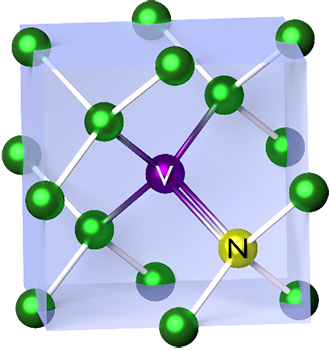
\includegraphics[width=0.3\linewidth]{figures/NV.png}
        \caption{The diamond cubic cell, where two adjacent carbon atoms have been substituted with a nitrogen and a vacancy. The double bond illustrates that there is an extra electron inside the vacancy. Image Credit: Wikimedia Commons}
        \label{fig:NV}
    \end{figure}
    In the world of quantum computing, these centers are especially promising as they have very long quantum coherence times at \textit{room temperature.} For context, many quantum computers need to be cooled down to near absolute zero. This is exciting as it opens up the possibility to room temperature quantum computing!

    In recent times, the coherence time has been increased from $2\si{\micro\second}$ in 2004\cite{best} all the way to one second in 2018\cite{Abobeih2018}. This $500,000$-fold increase in coherence time is caused by a better control of other impurities that may be present in diamonds during the doping process. Some of the popular methods used are described in the following section.
    \section{Doping Methods}
    \subsection{Annealing}
    In general, annealing is a thermal treatment where heating up a crystal lattice to very high temperatures can allow the migration of atoms, decreasing the \textit{dislocation density}.

    For diamonds in particular, it has been shown that annealing at temperatures above $600\si{\celsius}$ can cause carbon atoms to migrate into vacancies, thereby moving the vacancies around the lattice\cite{best}. These vacancies will end up at a more energetically favourable site such as beside the intrinsic nitrogen substitutional defects, forming $NV^{-1}$ sites. Specifically, the reaction:
    % https://www.mdpi.com/2504-4494/1/1/6/pdf
    \begin{equation}
        \ch{N+V->NV}
    \end{equation} 
    where \ch{V} is a vacancy, has a negative enthalpy change\cite{anneal}. However, the entropy change of the system is positive as there are less microstates $\Omega$ with the nitrogen dopant and vacancy adjacent to each other than microstates where they are randomly distributed. As a result, this reaction is only spontaneous at high temperatures. This explains why this migration only happens after the diamond is heated.
    
    % https://arxiv.org/pdf/1907.07793.pdf
    \begin{figure}[h]
        \centering
        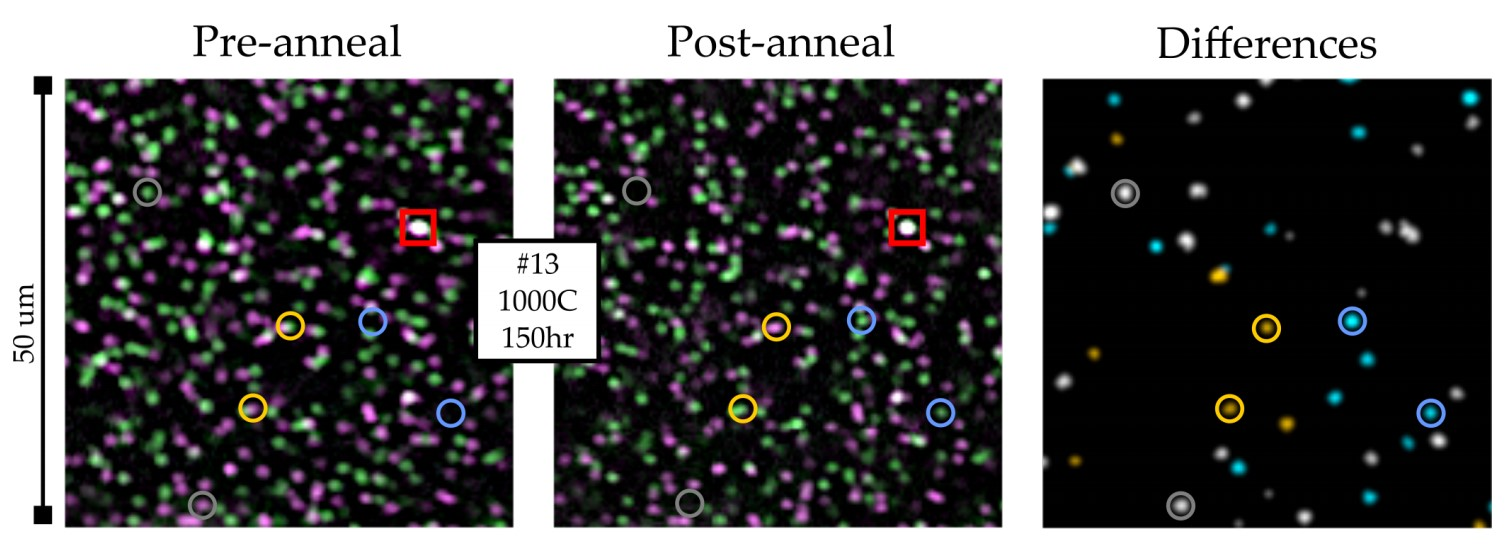
\includegraphics[width=0.8\linewidth]{figures/anneal.jpg}
        \caption{A comparison between before and after annealing was performed. The blue circles show the appearance of new $NV^{-}$ centers. Credit:\cite{Chakravarthi2020}}
        \label{fig:anneal}
    \end{figure}
    
    However, the limitation with this method is that the intrinsic dopants are distributed randomly and therefore difficult to control. This is not a big problem in many applications which only care about the existence of these sites, such as in gemology. However, in the quantum computing field, it is vital that we can create a precise number of $NV^{-}$ sites at predetermined locations.
    
    % https://arxiv.org/pdf/1907.07793.pdf
    \subsection{Direct Implantation}
    Direct Ion Implantation on the other hand, operates at low temperatures. The motivation behind ion implantation is to directly inject the desired ions into a material, and then annealing can be performed in a process known as \textit{post-annealing}.

    The general principle in traditional ion implantation is that the kinetic energy of the injected ions will exceed the binding energies of the target carbon atoms, creating a substitutional impurity. As a result, this technique is often very violent and can damage the target compound\cite{best}.

    This is not desirable when creating $NV^{-}$ sites at specific controllable locations in the diamond. This requirement lead to an entirely new method of direct implantation, which on top of being able to perform single ion implantation at low energies, it needs to satisfy the following two objectives\cite{Kalish2014}:
    \begin{itemize}
        \item Other unwanted defects introduced by the implantation must be removed around the ion site.
        \item Vacancies must be introduced surrounding the ion site.
    \end{itemize}
    We can model ion implantation as a series of collisions between the injected ion and the diamond atoms. This means the ion will gradually slow down until it reaches its final state as a substitutional impurity. During this process, collisions may break the bonds in the $sp^3$ hybridized carbon atoms and create vacancies. When the bonds reform, the carbon atoms will become $sp^2$ hybridized bonds instead, as double bonds are generally more stable. This process is known as \textit{graphitization} since the carbon atoms in graphite are $sp^2$ hybridized\cite{Kalish2014}. For certain applications, graphitization may be desired, but it is an unwanted side effect when working with quantum computers.
    
    While one may think that the vacancies created from these collisions can help form the $NV^{-}$ site, this is not the case. These ``side effect'' vacancies are often located at regions where the injected ion had a higher energy, which is typically far away from the final location of the ion\cite{Kalish2014}.
    \begin{figure}[h]
        \centering
        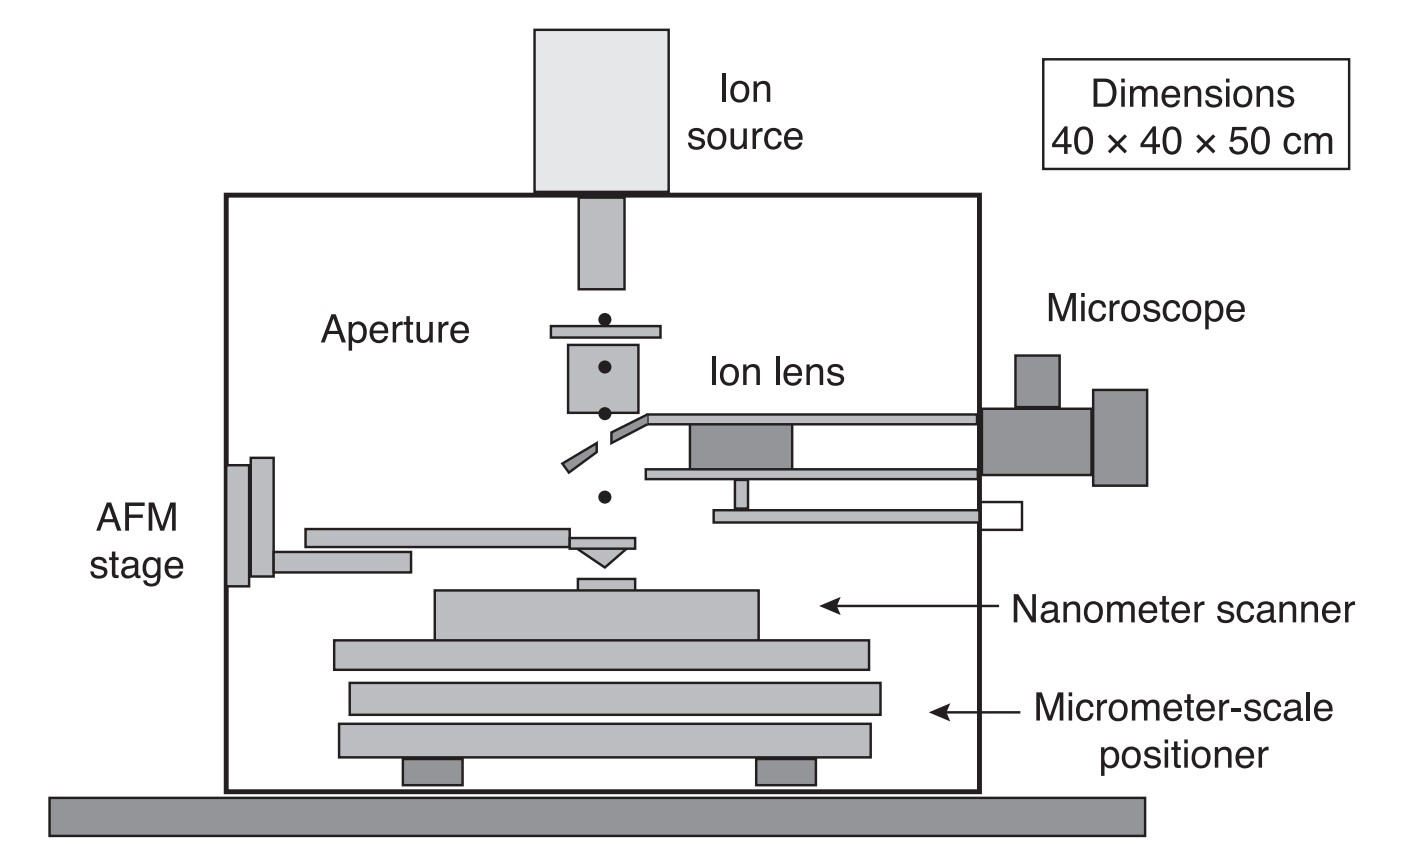
\includegraphics[width=0.7\linewidth]{figures/single-ion.jpg}
        \caption{An example schematic of what a single ion implantation device may look like. Credit: \cite{Kalish2014}}
        \label{fig:single-ion}
    \end{figure}

    Some of the damage from graphitization can be recovered from annealing, as going from a double to single bond increases the entropy so it is favourable at higher temperatures, but simulations show that if a damage density on the order of $1\times 10^{22} \text{ vacancies/cm}^3$ is reached, the damage cannot be repaired by annealing\cite{Kalish2014}.
    
    An example experimental apparatus to perform single-ion implantation is shown in figure \ref{fig:single-ion}. It consists of an ion beam and some sort of constriction device to limit the ion flow and to limit the kinetic energy of the ion to be the minimum needed to become a substitutional impurity.
    % file:///C:/Users/QiLin/Downloads/3-s2.0-B978085709656250003X-main.pdf

    While there has been some success achieving this, the aforementioned problems involving preventing residual damage and introducing vacancies at the same location has not been fully solved yet\cite{Kalish2014}.
    \section{Conclusion}
    The $NV^{-}$ color center makes diamonds a promising candidate when designing quantum computers, as they allow a long coherence time even at room temperature. The challenge researchers currently face is to carefully control and create these color centers at precise locations without damaging the rest of the diamond. However, progress in single-ion implantation is being made, and the future looks promising.
    \newpage
    \printbibliography


\end{document}

